\subsubsection{Tarjan (SCC em Uma Única Passada)}
O algoritmo de Tarjan encontra os SCCs utilizando apenas uma única DFS. Ele
mantém o tempo de descoberta de cada vértice (\textit{tin}) e o menor tempo
alcançável (\textit{low}). Utiliza uma pilha auxiliar para agrupar os nós
pertencentes ao mesmo componente conexo. Complexidade de tempo: $\mathcal{O}(V
    + E)$.

\paragraph{Pseudo-Código: }\mbox{}\\
\begin{algorithm}[H]
    \SetAlgoLined
    \SetKwFunction{Tarjan}{TarjanDFS}
    \SetKwProg{Fn}{Função}{:}{}

    \Fn{\Tarjan{$u, tin, low, pilha, naPilha, adj$}}{
        $tin[u] \gets low[u] \gets timer$\;
        $timer \gets timer + 1$\;
        $pilha.push(u)$\;
        $naPilha[u] \gets \text{true}$\;

        \For{$v \in adj[u]$}{
            \Se{$tin[v] == 0$}{
                \Tarjan{$v, tin, low, pilha, naPilha, adj$}\;
                $low[u] \gets \min(low[u], low[v])$\;
            }
            \Se{$naPilha[v]$}{
                $low[u] \gets \min(low[u], tin[v])$\;
            }
        }

        \Se{$low[u] == tin[u]$}{
            \text{// Encontrou a raiz de um SCC}\;
            \While{$topo \neq u$}{
                $topo \gets pilha.pop()$\;
                $naPilha[topo] \gets \text{false}$\;
                \text{adiciona $topo$ ao SCC atual}\;
            }
        }
    }
    \caption{Algoritmo de Tarjan para SCC}
\end{algorithm}

Veja o Tarjan utilizando tempos de descoberta e valores de \textit{low}:\\
\vspace{0.5cm} \noindent
\begin{minipage}[t]{0.31\textwidth}
    \centering
    \textbf{Passo 1: Descoberta ($tin, low$)}\\
    \vspace{0.2cm}
    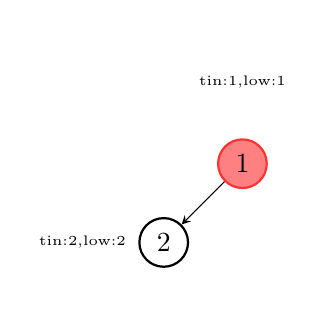
\begin{tikzpicture}[every node/.style={circle, draw, minimum size=0.5cm, thick}, >=stealth]
        \node[fill=red!50, draw=red!80, label=above:{\tiny tin:1,low:1}] (1) at (0, 1) {1};
        \node[label=left:{\tiny tin:2,low:2}] (2) at (-1, 0) {2};
        \draw[->] (1) -- (2);
    \end{tikzpicture}

    \vspace{0.2cm}
    \footnotesize
    \raggedright
    Visita o nó 1, define $tin[1]=low[1]=1$ e empilha. Vai para o nó 2.
\end{minipage}%
\hfill
%
\begin{minipage}[t]{0.31\textwidth}
    \centering
    \textbf{Passo 2: Back-edge e Low}\\
    \vspace{0.2cm}
    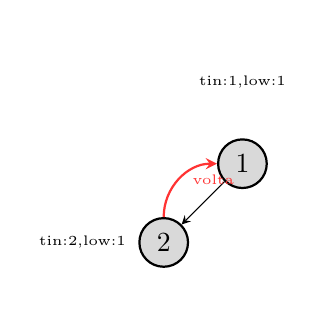
\begin{tikzpicture}[every node/.style={circle, draw, minimum size=0.5cm, thick}, >=stealth]
        \node[fill=gray!30, label=above:{\tiny tin:1,low:1}] (1) at (0, 1) {1};
        \node[fill=gray!30, label=left:{\tiny tin:2,low:1}] (2) at (-1, 0) {2};
        \draw[->] (1) -- (2);
        \draw[->, bend left=45, red!80, thick] (2) to node[right, draw=none, fill=none] {\tiny volta} (1);
    \end{tikzpicture}

    \vspace{0.2cm}
    \footnotesize
    \raggedright
    Aresta de retorno de 2 para 1 atualiza $low[2] = \min(low[2], tin[1]) = 1$.
\end{minipage}%
\hfill
%
\begin{minipage}[t]{0.31\textwidth}
    \centering
    \textbf{Passo 3: Raiz do SCC}\\
    \vspace{0.2cm}
    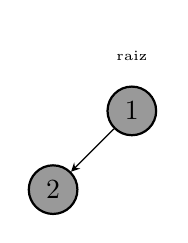
\begin{tikzpicture}[every node/.style={circle, draw, minimum size=0.5cm, thick}, >=stealth]
        \node[fill=gray!80, label=above:{\tiny raiz}] (1) at (0, 1) {1};
        \node[fill=gray!80] (2) at (-1, 0) {2};
        \draw[->] (1) -- (2);
    \end{tikzpicture}

    \vspace{0.2cm}
    \footnotesize
    \raggedright
    Como $low[1] == tin[1]$, 1 é raiz de um SCC. Desempilha os nós até 1.
\end{minipage}

\vspace{0.3cm}

\paragraph{Implementação: }\mbox{}\\
\textbf{C++:}
\begin{lstlisting}[language=C++]
int timer = 0;
void tarjanDFS(int u, const vector<vector<int>>& adj, vector<int>& tin, vector<int>& low, stack<int>& st, vector<bool>& inStack, vector<vector<int>>& sccs) {
    tin[u] = low[u] = ++timer;
    st.push(u);
    inStack[u] = true;
    
    for (int v : adj[u]) {
        if (tin[v] == -1) {
            tarjanDFS(v, adj, tin, low, st, inStack, sccs);
            low[u] = min(low[u], low[v]);
        } else if (inStack[v]) {
            low[u] = min(low[u], tin[v]);
        }
    }
    
    if (low[u] == tin[u]) {
        vector<int> comp;
        while (true) {
            int v = st.top(); st.pop();
            inStack[v] = false;
            comp.push_back(v);
            if (u == v) break;
        }
        sccs.push_back(comp);
    }
}
\end{lstlisting}
\newpage